\chapter{Photon Reconstruction in PandoraPFA}
\label{chap:Reconstruction}

\chapterquote{Photons have mass? I didn��t even know they were Catholic.}%
{Woody Allen}

\section{Introduction}{

Why photon reconstruction important.

\begin{comment}


Since the discovery of a particle consistent with being the SM Higgs boson in LHC at 2012 \cite{Aad:2012tfa,Chatrchyan:2012ufa}, our understanding of Standard Model has improved greatly. Yet limited by the underlying QCD interaction from proton-anti-proton collision, one has great difficulty to measure the properties of the Higgs precisely. Next generation electron-positron linear collider could hopefully make precision measurements of the Higgs sector and the Top quark sector \cite{Abramowicz:2013tzc}.

The leading candidates for next generation electron-positron linear collider are the International Linear Collider (ILC) \cite{Brau:2007zza}, and the Compact Linear Collider (CLIC) \cite{Linssen:2012hp}. The ILC has developed two detector models, namely the International Large Detector (ILD) \cite{Abe:2010aa} and the Silicon Detector (SiD) \cite{Aihara:2010zz}. The CLIC has developed two slightly modified detector models based on ILD and SiD \cite{Linssen:2012hp}. One key common feature of these next generation electron-positron linear colliders is the high granular calorimeter, which provides a great spatial resolution at the cost of the energy resolution. Particle flow algorithms (PFA) benefit from the spatial resolution from calorimeters, together with tracking information, to provide excellent a jet energy resolution. PandoraPFA, the most complicated and the best performing one, provides a jet energy resolution of less than 3.5\%, which is required for W/Z separation \cite{Thomson:2009rp,Marshall:2013bda}.

\begin{figure}[tbph]
\centering
{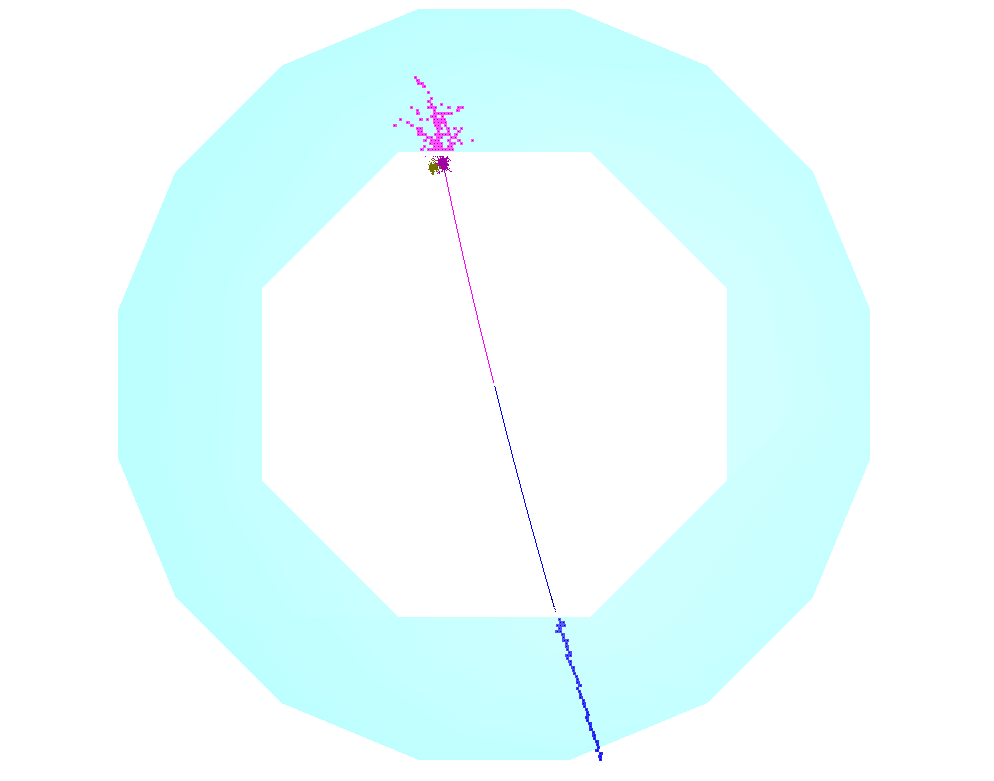
\includegraphics[width=0.5\textwidth]{images/tautauMod}}%

\caption{An event display of a simulated $\Pem\Pep\to \Ptauon\APtauon$ event. The blue region is the cross section of the Electromagnetic Calorimeter barrel region. The top $\Ptau$ decays into a charged $\Ppi$, two photons and neutrinos. The bottom $\Ptau$ decays into a muon and neutrinos.}
\label{fig:Tautau}
\end{figure}

Photon reconstruction is an important part of particle reconstruction. For many physics processes involving particles decaying into photons, such as $\Ptau$ lepton and $\Ppizero$, a good photon reconstruction, which provides a good single photon completeness and purity, as well as a good photon separation resolution, is crucial for reconstructing these particles.

\end{comment}
\section{Overview of photon reconstruction in PandoraPFA}

PandoraPFA provides a framework for particle reconstruction \cite{}, as described in \Section{}. In the linear collider content, it has a vast library of algorithms developed through years by many people. Each algorithm addresses one topological issue in the particle reconstruction \cite{}. The essential part of the PandoraPFA is track-cluster association and reclustering to find the best track-cluster pair. Algorithms that removes trackless clusters, such as removing muon clusters or photon clusters, would provide a clean environment for the track-cluster association, hence improving the jet energy resolution.

Photon identification in the PandoraPFA has two main mechanisms. The basic mechanism tests trackless clusters, the after track-cluster association and the reclustering processes. The second more sophisticated photon identification is performed before the track-cluster association and reclustering process. This algorithm identifies photon electromagnetic shower cores carefully in the dense jet environment.

Second mechanism improves jet energy resolution by correctly identifying photon electromagnetic shower cores and leaving a cleaner environment for the track-cluster association. However, the peripheral calorimeter hits to the shower cores may be left as fragments, and reconstructed as separate particles. This lowers the reconstructed photon completeness and makes the number of reconstructed photons a less useful physical quantity. Also, the second mechanism leaves rooms for improvement of photon separation resolution, illustrated in \Figure{}.

This section presents a solution to the photon fragments issue. The introduced PandoraPFA algorithms also improves the photon separation resolution. Algorithms related to photon reconstruction, fragmental removal and photon splitting, which are written or introduced by authors, will be discussed below.

%Three algorithm will be discussed: a rewritten sophisticated photon reconstruction algorithm, a photon fragment removal algorithm and a photons splitting algorithm.

%The testing simulated data in this paper are generated either by WHIZARD \cite{whizard} or by the simple HepEvt generator. Events are simulated with GEANT4 \cite{Agostinelli:2002hh} in MOKKA \cite{MoradeFreitas:2002kj}. Jet fragmentation was performed with PYTHIA \cite{Sjostrand:1995iq} and the particle reconstruction was done by PandoraPFA \cite{Marshall:2015rfa} in MARLIN reconstruction framework \cite{Gaede:2006pj}, in ILD\_o1\_v6 detector model. The iLCSoft v17-01-07 was used. Different versions of PandoraPFA were used for the comparison purpose.

\section{Overview of photon reconstruction algorithm}

The photon reconstruction algorithm refers to the more sophisticated photon identification of the two main identification mechanisms, before the track-cluster association and reclustering process. The algorithm has the following steps: coarsely forming photon clusters, reconstructing photon candidate, photon ID test, and optional fragment removals.

\subsection{Photon clusters}

This step finds large potential photon clusters. All calorimeter hits in the \ECAL, which are not used in previous algorithms, are grouped into clusters using a cone based clustering algorithm. To find photon clusters, which do not deposit energies in the tracking system, the cone clustering algorithm is seeded with energetic hits. The parameters for the cone clustering are generous, allowing potentially two or three photons in one cluster.

\subsection{Photon candidates}
\label{sec:photonCandiate}

The large photon clusters are split into smaller photon candidates, using two-dimensional shower profiles. The candidates close to a track projection are deemed as non-photons. Identifying photon candidates within a large photon cluster relies on the characteristic electromagnetic showers, in particular the transverse distribution. A energetic photon or electron hits the absorber layers of the \ECAL, it initiates an electromagnetic shower, where electron pair production and bremsstrahlung produce more low-energy photons and electrons. The transverse distribution is characterised by a narrow cone, widening while the shower develops.

To view the transverse shower distribution, a two-dimensional energy deposition projection is constructed in the plane perpendicular to the direction of the cluster. \Figure{fig:photonPeakFinding} shows the energy deposition projection of two photons candidates. U and V axis are two arbitrary orthogonal axis in the transverse plane perpendicular to the direction of photons. Z axis shows the sum of the calorimeter hit energy in GeV. The bin size corresponds to the square \ECAL cell size.

\begin{figure}[tbph]
\centering
{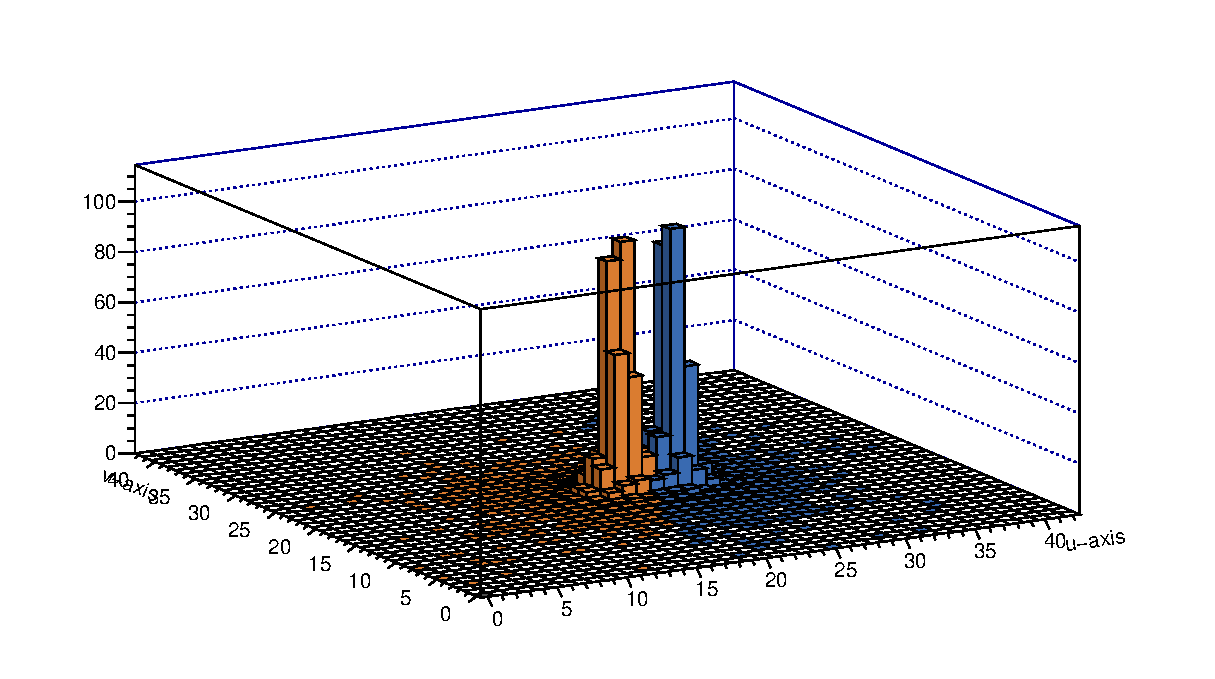
\includegraphics[width=0.5\textwidth]{photon/peakFinding}}%

\caption{Two 500\,GeV photons (yellow and blue), just resolved in the transverse plane perpendicular to the direction of the flight, of their energy deposition in electromagnetic calorimeter. U and V axis are two arbitrary axis perpendicular to each other in the plane. Z axis is the sum of the calorimeter hit energy in each particular bin in 2D plane in GeV.}
\label{fig:photonPeakFinding}
\end{figure}

By using the two-dimensional energy deposition projection, separating photons translates to separating peaks in the projection. Therefore a high performance two dimensional peak finding algorithm is the key to identify multiple photons. The peak finding algorithm will be discussed in \Section{sec:peakFinding}

The output of this step is a collection of photon candidates from a photon cluster, which will be fed to the photon ID test.

\subsection{Photon ID test}

Photon ID test decides if a a candidate is a photon. If a candidate is not a photon, the calorimeter hits of the candidate will be passed on to the next stage of the reconstruction.  The photon ID test is a multidimensional likelihood classifier. The classifier is trained with discriminating variables, which exploit features electromagnetic showers. The classifier will be discussed in \Section{}

\subsection{Photon Fragment removal}

The optional photon fragment removal aims to merge small photon fragment to main photons. Since this step shares the same logic as the algorithm in \Section{}, only differing in the cut-off values for merging in the metrics, this step be discussed in \Section{}.

This step marks the end of the photon reconstruction algorithm. The output are a collection of reconstructed photons, separated from non-photon calorimeter hits.
%The candidate passed the test will be kept in a separate container for photons only

\section{Two dimensional peaking find algorithm for photon candidate}
\label{sec:peakFinding}

As discussed in \Section{sec:photonCandiate}, separating photon candidates from a cluster is same as identifying peaks in a two dimensional histogram. An example of two photons is shown in the \Figure{fig:photonPeakFinding}. The basic algorithm treats all clusters as potential photon clusters. Since charged hadrons would deposit tracks in the tracking system, extra care is taken when a cluster is close to the projection of the track in the front of the \ECAL. The basic peak finding algorithm has two main functions: identifying peaks, and assigning bins to peaks.

A local peak is defined as a bin where its height is above all eight neighbouring bins. After all peak bins are found, non-peak bins are associated to one peak bin, by choosing the peak bin that gives the minimal metric
\begin{equation}
\frac{d}{\sqrt{E_{peak}}}}
\end{equation}
where $d$ is the Euclidean distance between a non-peak bin and a peak bin, and $E_{peak}$ is the energy or the height of the peak bin. Alternative metrics provided in the algorithm include
\begin{equation}
\frac{d}{\sqrt{E_{peak}}}},
\end{equation}
\begin{equation}
\frac{d}{{E_{peak}}},
\end{equation}
\begin{equation}
\frac{d}{{E_{peak}^2}}
\end{equation}
The default metric is chosen due to a good balance between distance and energy of the peak.

\subsection{Candidate close to track projection}

If a cluster or a photon candidate is close to the projection of the track in the front of the \ECAL, it is likely that the cluster or the candidate is a charged hadron. Misidentifying a charged hadron as a photon leads to significant degradation in reconstruction performance. However, if a photon next to a charged hadron is carefully reconstructed, the overall reconstruction is improved. Hence this step aims to carefully identifies photon candidate next to charged hadrons, by using track information and features of the electromagnetic shower. Photon induced electromagnetic shower in the \ECAL typically start in the first few layers. As the shower develops, the direction of the shower core does not change much.

If a peak bin is within the eight neighbouring bins of the track projection onto the two dimensional plane, the peak and its associated bins are flagged as non-photons. Furthermore, the \ECAL is sliced longitudinally to help identify photon candidates. For example, the default three slices will result in three \ECAL fiducial spaces, each contains space from the front of the \ECAL to a third, two thirds and the back of the \ECAL, respectively. The peaking finding algorithm is repeated for the same cluster divided in each \ECAL fiducial space. The peak is only preserved as a photon candidate if the peak exists in every fiducial space, and if its position is shifted by no more than one neighbouring bin between fiducial spaces.


\subsection{Speed and performance tuning}

The bin is 


The default histogram size is 41 by 41 bins. 



The input of the two dimensional peak finding algorithm is a two dimensional histogram. 


\section{Likelihood classifier for photon ID}
Discriminating variables of each candidate are calculated. The variables are used for trainning the classifier and for the classification.













\begin{comment}
When a high-energy electron or photon is incident on a thick absorber, it initiates
an electromagnetic cascade as pair production and bremsstrahlung generate more
electrons and photons with lower energy.

The longitudinal development is governed by
the high-energy part of the cascade, and therefore scales as the radiation length in the
material. Electron energies eventually fall below the critical energy, and then dissipate
their energy by ionization and excitation rather than by the generation of more shower
particles.

The distributions
are characterized by a narrow core, and broaden as the shower develops. They are often
represented as the sum of two Gaussians,
\end{comment}
%The core part of the standalone photon reconstruction algorithm is to identify peaks in a 2D plane, the energy deposition of a transverse 2D plane perpendicular to the direction of the flight. Each identified peak will form a cluster. The cluster will be identified as a photon if it passes the photon likelihood test. The key to improve photon separation resolution is to improve the 2D peak finding algorithm. We have implemented a new peak finding algorithm, which finds all possible local maxima. Other cells in the 2D plane are associated to each peak by minimising the metric $d/\sqrt(E)$, where $d$ is the distance in 2D plane from the cell to the peak, and $E$ is the energy or height of that particular peak. \Fig{fig:peakFinding} shows two energetic photons just resolved with the new 2D peak finding algorithm.


%The standard reconstruction reconstructs muons before this step. Hence ideally the hits in the \ECAL belong to photons or charged hadrons.

